\documentclass[UTF8]{ctexart}

\usepackage[linesnumbered,boxed,ruled,commentsnumbered]{algorithm2e}
\usepackage{bm}
\usepackage{graphicx}
\usepackage{float}
\usepackage[bookmarks=true]{hyperref}
\usepackage{amsmath}
\begin{document}
\title{数值分析大作业一报告}
\author{陈昭熹 2017011552}
\maketitle

\section{问题分析}

\subsection{问题分解}

\subsubsection{必做任务}

必做任务要求将给定尺寸为$512 \times 512$以图片中心像素点进行旋转扭曲。该任务可以被分解为以下三步:
\begin{itemize}
    \item 图片读取与预处理
    \item 计算新图中扭曲点在原图中的坐标位置
    \item 依照原图中的浮点坐标位置对像素值进行插值
    \item 显示扭曲后的图像
\end{itemize}

\subsubsection{选做任务}
选做任务要求利用薄板样条插值(Thin Plate Spline),在给定的人脸图像之间,利用预先给出的68个人脸特征控制点进行变形,达到人脸融合的效果。该任务可以被分解为以下几步:
\begin{itemize}
\item 图片预处理与特征点读取
\item 求解原图到目标图的TPS坐标变换矩阵
\item 利用坐标变换矩阵对目标图中所有像素点进行坐标变换
\item 在原图中用变换得到的坐标插值出像素值
\item 显示变形后的图像
\end{itemize}

\subsection{需求分析}

\subsubsection{必做任务}
依照上面的问题分解,必做任务中的坐标转换已经预先给出,因此只需要实现插值函数。按照要求,本次将实现最近邻、双线性、双三次三种插值方法。

\subsubsection{选做任务}
选做任务是一个更为复杂的应用场景,因此所需要考虑的细节也就更多。建立在必做任务中所实现的插值方法基础上,本任务中需要实现TPS变形的求解器。同时针对TPS全局变形的特点,变形后的图片有可能与原图尺寸相差很远,若继续用原图尺寸显示,则会在图片四周产生大量黑色像素,有碍观感,因此需要实现边缘裁剪等功能。

\section{方案设计}

\subsection{基本原理}

\subsubsection{插值函数}
令$I(x,y)$表示某点处的像素值,本文实现了如下三种插值函数:

\begin{itemize}
    \item [\textbf{最近邻}]

    最近邻插值对于给定的插值节点,选择距离其最近的像素点的像素值作为其自身的像素值。在本文实现过程中,使用待插值节点的左上角点的像素值。
    $$I(x',y')=I(\lfloor x+0.5 \rfloor,\lfloor y+0.5 \rfloor)$$
    \item [\textbf{双线性}]
    
    双线性插值对于给定的插值节点,选择距离其最近的四个像素点,分别从x轴和y轴两个方向进行线性插值,并将两次线性插值的结果加权后作为最终结果。在本文实现中,选取待插值节点周围最近的四个点,即该节点被四个插值节点构成的方格所围住。具体实现如下,$待插值点坐标为(x,y)$,使用的四个插值节点为:
    \begin{equation}
        \begin{cases}
            p_1 = (\lfloor x \rfloor , \lfloor y \rfloor)\\
            p_2 = (\lfloor x \rfloor, \lfloor y \rfloor +1)\\
            p_3 = (\lfloor x \rfloor +1, \lfloor y \rfloor)\\
            p_4 = (\lfloor x \rfloor +1, \lfloor y \rfloor +1)
        \end{cases}
    \end{equation}
    返回的像素值通过下面的插值函数计算出来:
$$
        I(x',y')=\frac{1}{(x_2-x_1)(y_2-y_1)}
        \left[
        \begin{matrix}
            x_2-x & x-x_1
        \end{matrix}    
        \right]
        \left[
        \begin{matrix}
            I(p_1) & I(p_2)\\
            I(p_3) & I(p_4)
        \end{matrix}    
        \right]
        \left[
        \begin{matrix}
            y_2-y\\
            y-y_1
        \end{matrix}    
        \right]
$$
    其中,$(x_1,y_1)=p_1, (x_2,y_2)=p_4$。

    \item [\textbf{双三次}]
    
    双三次插值不同于前面的两种线性方法,通过一个核函数来计算插值节点信息,同时使用到的插值节点更多,达到了16个,将待插值点放置在一个4x4网格中,具体方法定义如下:
    \begin{equation}
        \begin{cases}
            u=x-\lfloor x\rfloor\\
            v=y-\lfloor y\rfloor
        \end{cases}
    \end{equation}
    \begin{equation}
        A = \left[
        \begin{matrix}
            BK(1+v) & BK(v) & BK(1-v) & BK(2-v)\\
        \end{matrix}    
        \right]^T
    \end{equation}
    \begin{equation}
        C = \left[
        \begin{matrix}
            BK(1+u) & BK(u) & BK(1-u) & BK(2-u)\\
        \end{matrix}    
        \right]^T        
    \end{equation}
    其中函数$BK(x)$为双立方核函数,定义如下:
    \begin{equation}
        BK(x)=\begin{cases}
            (a+2)|x^3|-(a+3)|x^2|+1, |x|\leq 1\\
            a|x^3|-5a|x^2|+8a|x|-4a, 1<|x|<2\\
            0, |x|\geq 2
        \end{cases}
    \end{equation}
在本文的实现中,BK为一元函数,其中\textbf{a取常数-1}。利用十六个插值节点的像素值,可以构造:
$$
    B=\left[\begin{array}{cccc}{I(\lfloor x\rfloor- 1,\lfloor y\rfloor- 1)} & {I(\lfloor x\rfloor- 1,\lfloor y\rfloor)} & {I(\lfloor x\rfloor- 1,\lfloor y\rfloor+ 1)} & {I(\lfloor x\rfloor- 1,\lfloor y\rfloor+ 2)} \\ {I(\lfloor x\rfloor, l y-1)} & {I(\lfloor x\rfloor, \lfloor y\rfloor)} & {I(\lfloor x\rfloor, L y\rfloor+ 1)} & {I(\lfloor x\rfloor,\lfloor y\rfloor+ 2)} \\ {I(\lfloor x\rfloor+ 1,\lfloor y\rfloor- 1)} & {I(\lfloor x\rfloor+ 1,\lfloor y\rfloor)} & {I(\lfloor x\rfloor+ 1,\lfloor y\rfloor+ 1)} & {I(\lfloor x\rfloor+ 1, \lfloor y\rfloor+ 2)} \\ {I(\lfloor x\rfloor+ 2, l y\rfloor- 1)} & {I(\lfloor x\rfloor+ 2, l y)} & {I(\lfloor x\rfloor+ 2,\lfloor y\rfloor+ 1)} & {I(\lfloor x\rfloor+ 2,\lfloor y\rfloor+ 2)}\end{array}\right]
$$

最终给出插值结果:$I(x',y')=ABC^T$
\end{itemize}

\subsubsection{图像中心扭曲(切向畸变)}
设新图像的整数型坐标$(x',y')$,对应原图像的浮点型坐标$(x,y)$,畸变控制参数为最大旋转角度$a_{max}$和扭曲旋转半径$Radius$,对应到每一个点旋转的角度为:
$$a=a_{max}\times \frac{Radius-Distance}{Radius}$$

其中$Distance$为坐标$(x',y')$到图像中心点的距离。\textbf{基于这样的模型我们在该问题中应当使用图像中心坐标系进行计算,最后在转到像素坐标系中进行实现。}此时根据数学推导可得:
\begin{equation}
    \begin{cases}
    x=x'cosa - y'sina\\ 
    y=x'sina+y'cosa
    \end{cases}
\end{equation}

根据此可以计算出扭曲后的图像的网格点上对应原图的浮点坐标,再通过插值可以得到相应的像素值,从而完成图像扭曲。

\subsubsection{图像径向畸变}

图像径向畸变一般指的是桶形畸变和枕型畸变,分别对应着图像平面从观感上向观察者凸起或者凹陷的畸变。在大作业的课上讲解中使用了球面模型来建模这样的畸变,但是在本文的实现中,并未采取这种繁琐的模型。事实上,径向畸变起源于相机镜头是曲面的,往感光平面上投影时势必会产生误差,具体体现为离相机中心远的像素具有更大的放大率,而距离近的则近似不移动,总体看从相机中心出发呈现径向上的差异。受到畸变产生原理的启发,本文在实现过程中直接在平面上进行操作,通过定义径向畸变率$distortion_K$来模拟相机镜头投影到平面上的不同的变形作用,令其作为不同像素点到图像中心距离的权重来进行坐标变换,从而在平面上实现了径向畸变。值得注意的是,变换过程中需要进行两次坐标系转化,从像素坐标系变换到相机坐标系(即图像中心为原点),计算畸变后还原到像素坐标系中以便于插值。设新图像在像素坐标系下的整数型坐标$(x'_p,y'_p)$,在相机坐标系下的坐标为$(x'_c,y'_c)$;对应原图像在像素坐标系下的浮点型坐标$(x_p,y_p)$,在相机坐标系下的坐标为$(x_c,y_c)$。受到相机畸变模型的启发,将上一节所使用的半径$Radius$沿用下来,定义为畸变半径,其物理意义就是相机模型中的相机焦距$(f_x,f_y)$,由于本文重点在于做图像畸变,而非相机畸变矫正,因此将两个方向的焦距均取为$Radius$,便于实现。下面给出具体的坐标变换公式:
\begin{equation}
    \begin{cases}
        x_c = \frac{x'_c}{Radius} \cdot (1+distortion_K \cdot Distance^2)\\
        y_c = \frac{y'_c}{Radius} \cdot (1+distortion_K \cdot Distance^2)\\
        (x_p,y_p) = (x_c,y_c)\cdot Radius + centre
    \end{cases}
\end{equation}

其中$centre$为图像中心点在像素坐标系下的坐标,通常各取为图像长宽的一半。

\subsubsection{TPS网格变形}
TPS即薄板样条变形,其主要目标是寻找一个通过所有控制点的光滑曲面$f(x,y)$,使得能量函数If最小,能量函数定义与求解过程无关,在此不进行赘述。下面给出TPS求解过程:
给定n个控制点$$\{P_1=(x_1,y_1),\dots,P_n=(x_n,y_n)\}$$

假设目标点为$$\{ \tilde{P_1}=(x'_1,y'_1),\dots,\tilde{P_n}=(x'_n,y'_n)\}$$

定义如下辅助变量:
\begin{equation}
    K=\left[
    \begin{matrix}
        0 & U(r_{12}) & \dots & U(r_{1n})\\
        U(r_{21}) & 0 & \dots & U(r_{2n})\\
        \dots & \dots & \dots & \dots \\
        U(r_{n1}) & U(r_{n2}) & \dots & 0
    \end{matrix}    
    \right]
\end{equation}
\begin{equation}
    P=\left[
    \begin{matrix}
        1 & x_1 & y_1 \\
        1 & x_2 & y_2 \\
        \dots & \dots & \dots \\
        1 & x_n & y_n
    \end{matrix}    
    \right]
\end{equation}
\begin{equation}
    L=\left[
    \begin{matrix}
        K & P\\
        P^T & \textbf{0}
    \end{matrix}    
    \right]
\end{equation}
\begin{equation}
    V=\left[
    \begin{matrix}
        x'_1 & x'_2 & \dots & x'_n\\
        y'_1 & y'_2 & \dots & y'_n
    \end{matrix}    
    \right]
\end{equation}
\begin{equation}
    Y=\left[
    \begin{matrix}
        V_1 & 0 & 0 & 0\\
        V_2 & 0 & 0 & 0
    \end{matrix}
    \right]^T
\end{equation}
\begin{equation}
    L\left[
    w_1,\dots,w_n,a_1,a_x,a_y    
    \right]^T = Y
\end{equation}

则所拟合出的光滑曲面(即一个关于xy的二元函数,函数值对应着像素点的像素值):
\begin{equation}
    f(x,y)=\left[
    f_x(x,y),f_y(x,y)    
    \right]^T
    =a_1+a_xx+a_yy+\Sigma w_iU(|P_i-(x,y)|)
\end{equation}

值得注意的是,其中定义了径向基函数$$U(r)=\begin{cases}
    r^2log(r^2),r\neq0\\
    0,r=0
\end{cases}
$$

这个函数直观的给出了控制点周围的变形插值函数,不同的距离体现了不同的变形效果。

需要澄清的一点是,本文实现中,控制点来源于目标图片(target image),而目标点来源于源图片(original image),这一点在代码中是容易混淆的。由于TPS属于全局变形,虽然人脸的68个控制点会集中在图片中一个小区域,但是经过能量最小化处理后,图片的边界可能会缩入原图尺寸之内,导致边缘部分出现很多黑色像素。这样的情况在变形的两张图片之间尺寸差别很大的时候会十分明显,因此为了观感,需要进行\textbf{图片裁剪}。图片裁剪的原理也就基于这样的现象,对于变换后的图片从四个边界向内部归并搜索,遇到黑像素则缩小边界。迭代结束后去最大的边界作为裁剪后的尺寸。

\subsection{UI设计与向导}

\subsubsection{界面概览}
\begin{figure}[H]
    \centering
    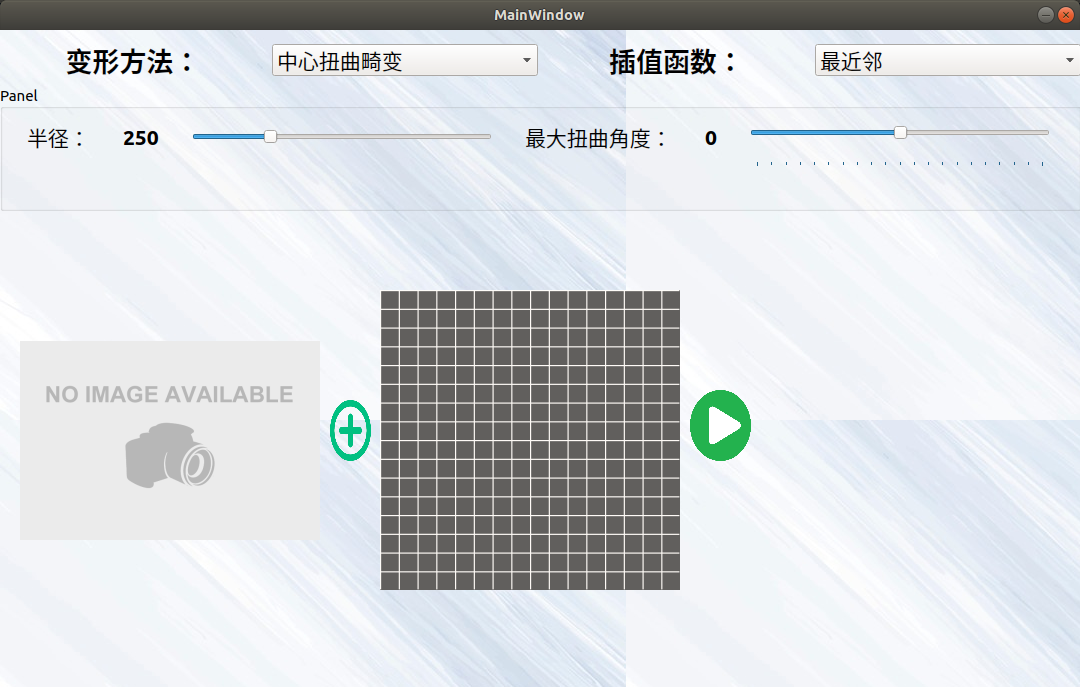
\includegraphics[scale=0.3]{images/report-images/manual.png}
    \caption{用户界面}
\end{figure}

\subsubsection{使用方法}
\begin{itemize}
\item 选择变形方法:左上侧下拉框选择
\item 选择插值函数:右上方下拉框选择
\item 选择源图片:点击第一个Image提示按钮,选择文件路径
\item 选择目标图片(仅限于TPS变形):点击第二个Image提示按钮,选择文件路径
\item 开始变形/畸变:点击绿色的开始按钮
\item 更改畸变参数(仅限非TPS变形):在Panel中进行拖动更改,当拖动改变相应参数后,会在第二个图片框中利用黑色背景的网格实时显示当前的变形效果,便于用户直观观察。
\end{itemize}


\section{结果分析}

\subsection{图像处理效果}

\subsubsection{各畸变的实现}
\begin{figure}[H]
    \centering
    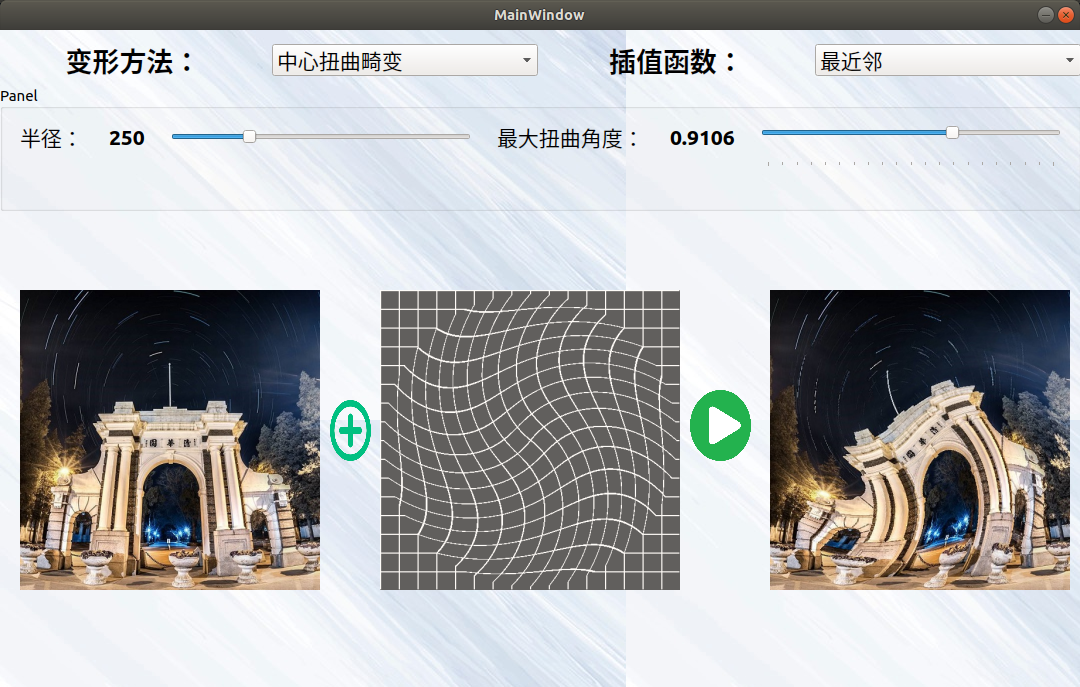
\includegraphics[scale=0.3]{images/report-images/tangent_dis.png}
    \caption{中心旋转畸变}
\end{figure}
\begin{figure}[H]
    \centering
    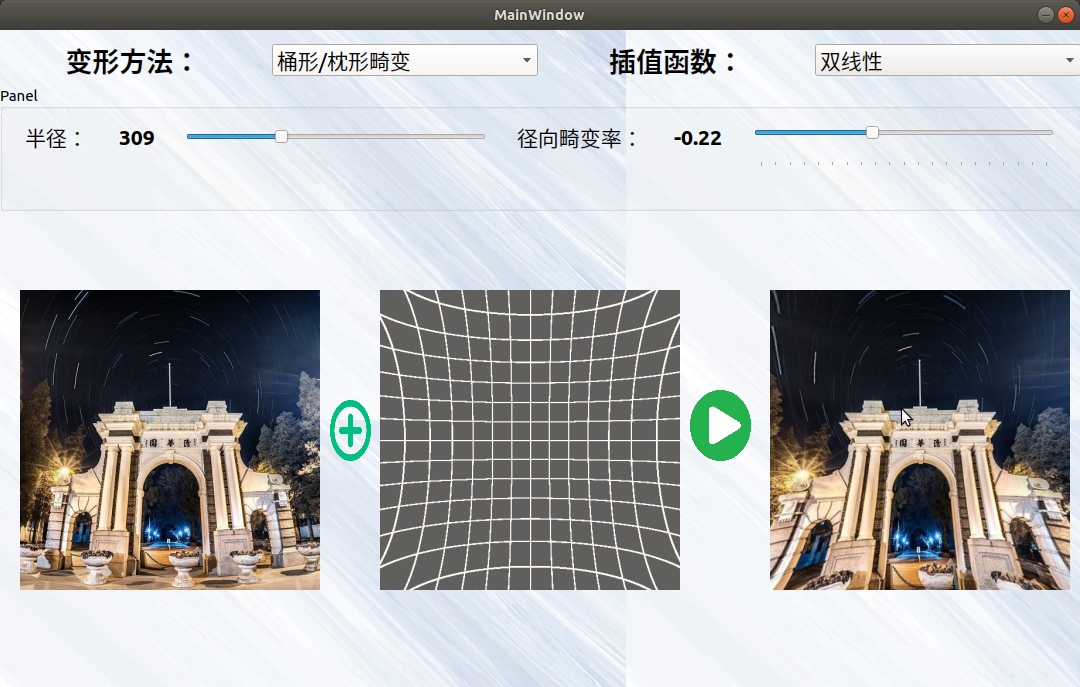
\includegraphics[scale=0.3]{images/report-images/ao.png}
    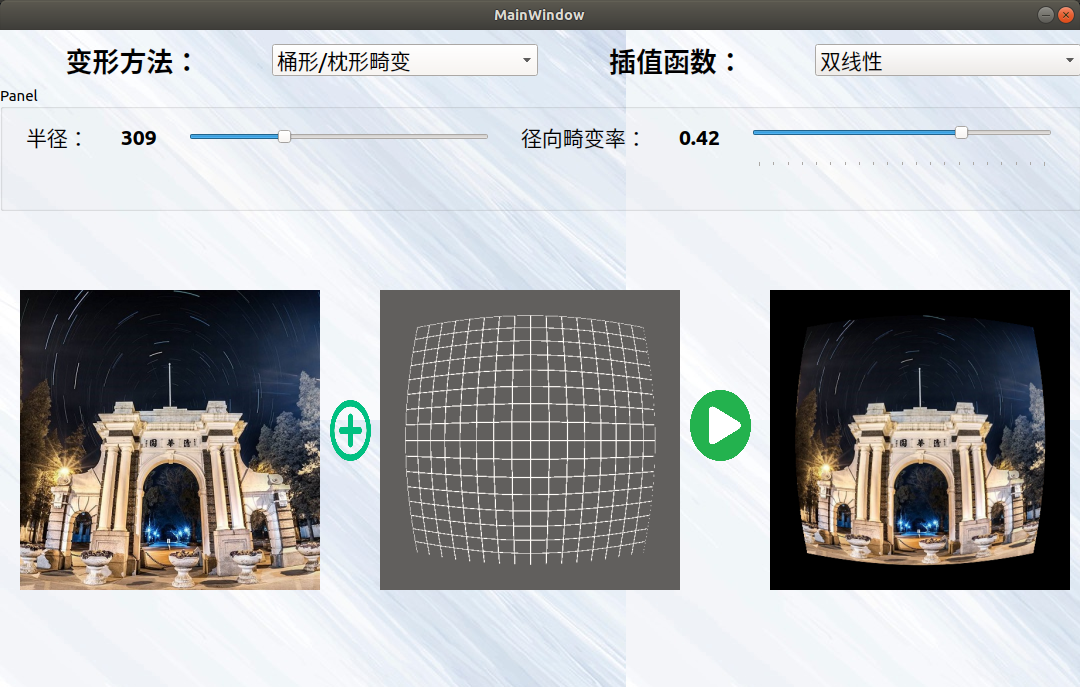
\includegraphics[scale=0.3]{images/report-images/tu.png}
    \caption{径向畸变}
\end{figure}
\begin{figure}[H]
    \centering
    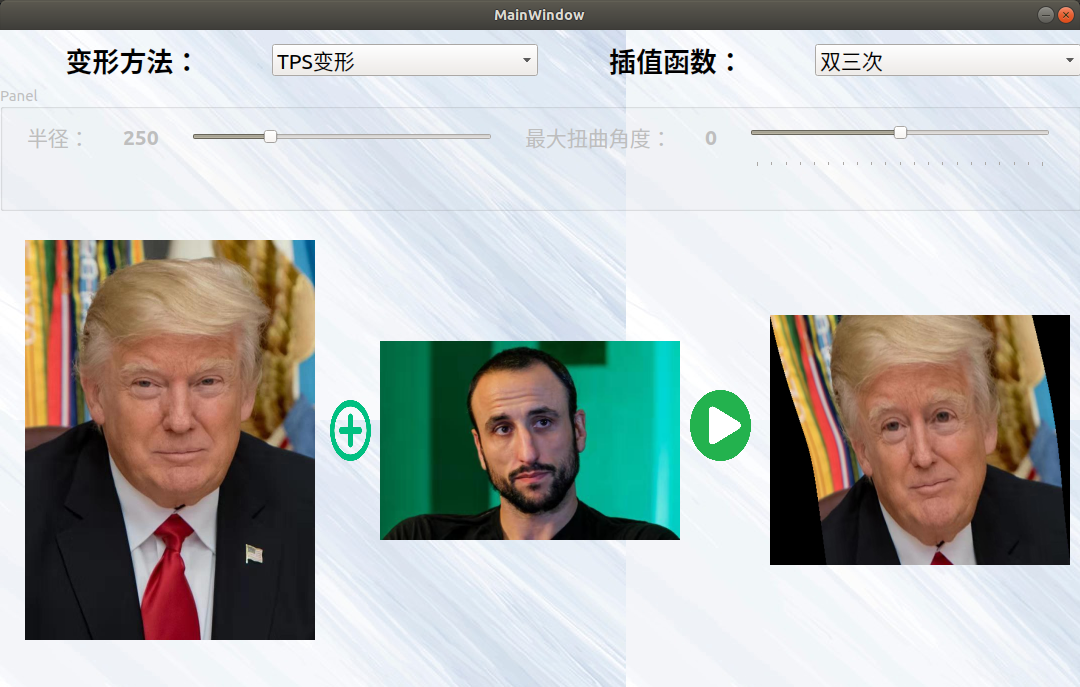
\includegraphics[scale=0.3]{images/report-images/trump.png}
    \caption{TPS}
\end{figure}

\subsubsection{不同插值函数的表现}
总体来看,三种插值函数表现大致相同,但计算速度上最近邻最快,双线性次之,双三次最慢。值得注意的是在一些极限情况下,双三次能够更好的将图像细节还原,而低阶次的插值会出现明显的锯齿感,以二校门顶端的金属直杆在大角度旋转情况下尤为明显。

\begin{figure}[H]
    \centering
    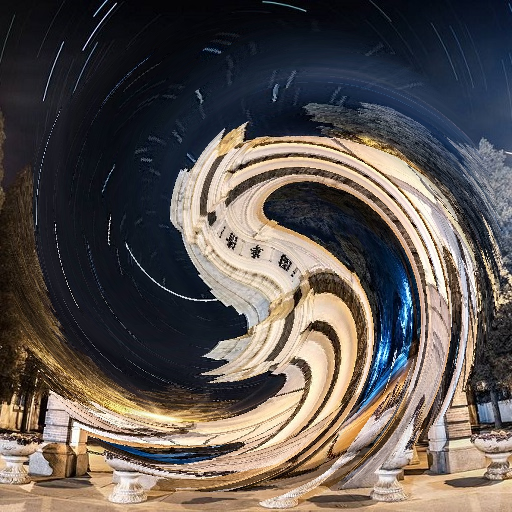
\includegraphics[scale=0.2]{images/report-images/tangent_distortionnearest.png}
    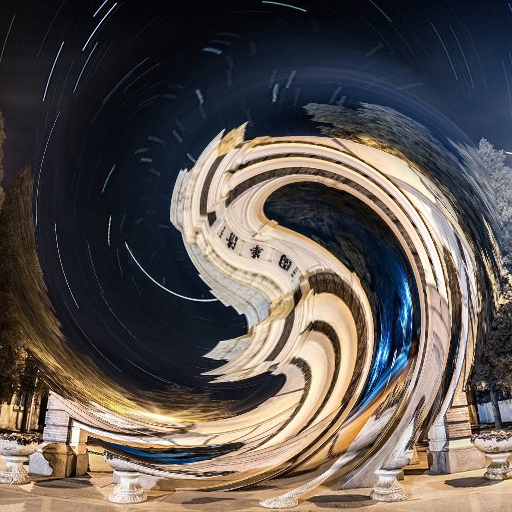
\includegraphics[scale=0.2]{images/report-images/tangent_distortionbilinear.png}
    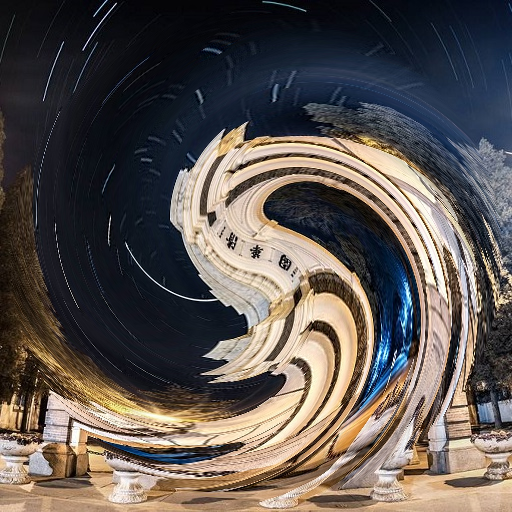
\includegraphics[scale=0.2]{images/report-images/tangent_distortionbicub.png}
    \caption{中心旋转畸变:最近邻-双线性-双三次}
\end{figure}

\begin{figure}[H]
    \centering
    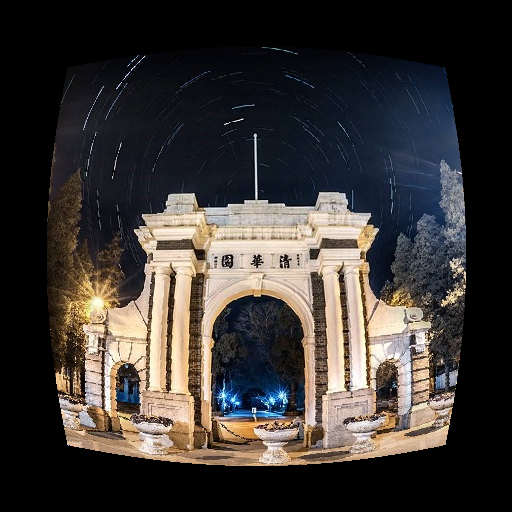
\includegraphics[scale=0.2]{images/report-images/radical_distortionnearest.png}
    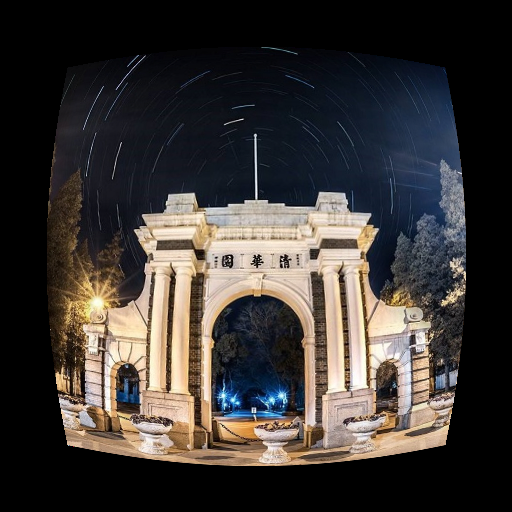
\includegraphics[scale=0.2]{images/report-images/radical_distortionbilinear.png}
    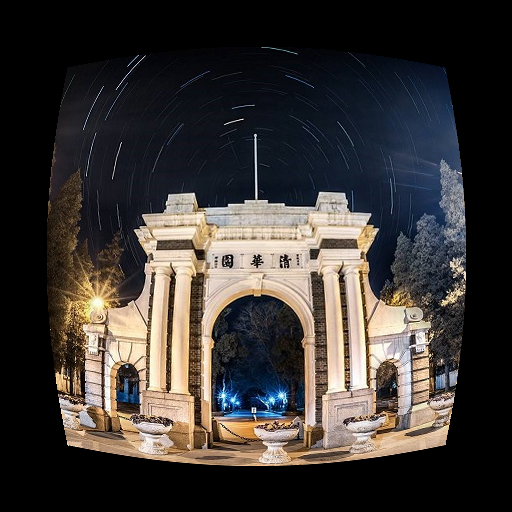
\includegraphics[scale=0.2]{images/report-images/radical_distortionbicub.png}
    \caption{径向畸变:最近邻-双线性-双三次}
\end{figure}

\begin{figure}[H]
    \centering
    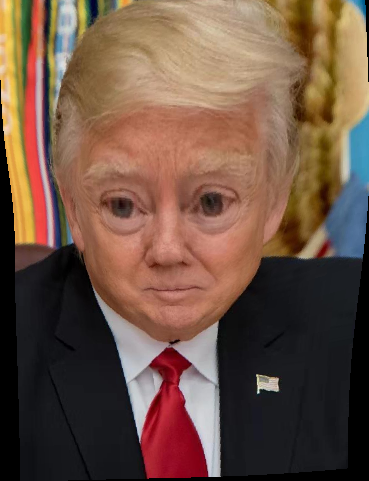
\includegraphics[scale=0.28]{images/report-images/8to6nearest.png}
    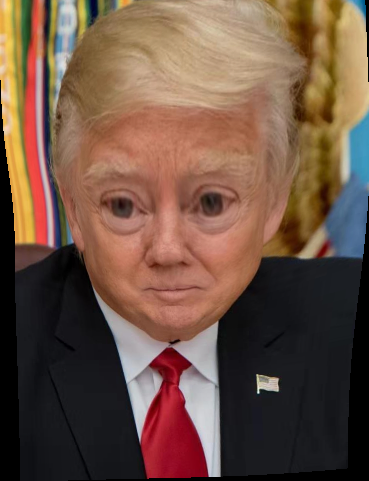
\includegraphics[scale=0.28]{images/report-images/8to6bilinear.png}
    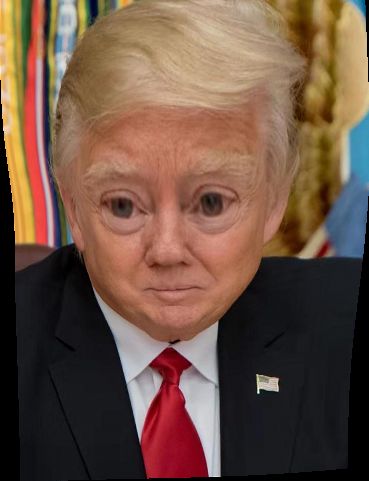
\includegraphics[scale=0.28]{images/report-images/8to6bicub.png}
    \caption{TPS人脸变形:最近邻-双线性-双三次}
\end{figure}


\subsection{误差分析}
误差分析部分主要针对舍入误差和插值函数产生的误差进行分析。
\subsubsection{舍入误差}
舍入误差主要是在计算机处理图像时产生的。主要产生在\textbf{像素值的处理和坐标值的处理}中。

首先是由于数字图像在产生的时候是通过对RGB三个通道的像素离散采样而得到的,在本文语境下,使用CV\_8U3C结构来存储图像意味着每一个通道像素值为0~255,采样间隔为1,因此这部分的舍入误差$\leq 1/2$。

其次在从目标图像的整数像素点到原图像的浮点像素点的坐标转换过程中,使用double类型来存储坐标值,由于double类型表示最大位数为16位,因此每一次计算均会产生$10^{-16}$的误差。这个数量级的误差在本文情境下基本可以忽略。


\subsubsection{方法误差}
\begin{itemize}
\item [\textbf{最近邻}]
显然最近邻的取整处理会使得这种方法在x,y两个方向均产生$|\Delta x|\leq \frac{1}{2},|\Delta y|\leq \frac{1}{2}$,由于像素值是关于xy的二元函数,即$I(x,y)$,因此其误差可以由此计算出来:
$$|\Delta I(x,y)| \leq max|\frac{\partial I}{\partial x}|\cdot|\Delta x| + max|\frac{\partial I}{\partial y}|\cdot||\Delta y| = \frac{1}{2}(max|\frac{\partial I}{\partial x}|+max|\frac{\partial I}{\partial y}|)$$
\item [\textbf{双线性}]
双线性插值可以看做x,y两个方向上的线性插值,由于两个方向上是不相关的,因此其误差可以分解为两个方向单线性插值的叠加。由线性插值的余项:
$$|R_1(x)|\leq \frac{M_2}{2} |x-x_0||x-x_1|$$

在本文实现中,上式的$x_0,x_1$分别是$\lfloor x \rfloor, \lfloor x \rfloor+ 1$,代入到上面余项公式中可以明显的看到后面两项是一个对勾函数,当x取值为在两个插值节点的中点时有最大值1/4,因此可以进行如下放缩:
$$|R_1(x)|\leq \frac{M_2}{8}$$

而$M_2 = max|\frac{\partial^2I}{\partial x^2}|$,因此对于双线性插值其总体误差可以用下式表示:
\begin{equation}
    |R| \leq \frac{1}{8}(max|\frac{\partial^2 I}{\partial x^2}|+max|\frac{\partial^2 I}{\partial y^2}|)
\end{equation}

\item [\textbf{双三次}]
借鉴上面求取双线性插值误差的方法,这里双三次插值从原理上也可以看做是两个方向上的三次样条插值,由三次样条插值余项定义:
$$|R(x)|\leq \frac{5}{384} M_4(\frac{b-a}{n})^4$$其中$b-a$为区间长度,$n+1$为插值节点数,$M_4=max|\frac{\partial^4 I}{\partial x^4}|$因此在本文实现方法中$b-a=3,n=4-1=3$,因此有$$|R(x)|\leq \frac{5}{384}max|\frac{\partial^4 I}{\partial x^4}|$$

故对于双三次插值其总体误差可以用下式表示:
\begin{equation}
    |R| \leq \frac{5}{384}(max|\frac{\partial^4 I}{\partial x^4}|+max|\frac{\partial^4 I}{\partial y^4}|)
\end{equation}
\end{itemize}
\section{总结与体会}
本次大作业任务虽重,但带来的收获无疑是巨大的。

首先,我对于图像处理问题中常见的坐标系统以及坐标转换关系有了一个深刻的认识,也认识到具体实现过程中OpenCV的坐标系统与数据结构存储中的变换关系(即x=col=width,y=row=height)。同时我也对于图像处理的一些基本思想、基本方法有了一个初步的认识,这将会对我之后的学习大有帮助。

其次,这次大作业也极大地锻炼了我在实现图像问题时的工程实践和解决问题的能力。通过前后端分离的方式,结合GDB高效的断电操作以及内存监控,我能够快速地诊断到代码中究竟是哪里让图像没有达到我想要的效果,这在处理庞大矩阵时个别点数据不可观的情况下是极其有用的经验技巧。

尽管最后在前后端通信上没有采用基于内存的方式,而是采用基于文件的方式,但是我还是尝试着实现了Qt中的图像系统与OpenCV中的图像系统之间的转换,即QImage与cv::Mat之间的转换,这也让我对于深拷贝、浅拷贝、多通道图像、图像矩阵在内存中的真实存放方式有了更深一步的理解。

最重要的一点是,通过此次大作业我在实践中对于插值方法与误差掌握地更加熟练,也认识到在实现中针对不同插值函数的特点和误差要求需要选择合适方法,有时候最近邻也不一定是最差的,双三次也不一定是最好的。

最后,感谢助教和老师的悉心指导和帮助!

\end{document}